\chapter{PC aplikace}

K obsluze zařízení sice postačí textový terminál sériové linky, 
ale pro pohodlné používání a automatizované funkce je vhodné použít doprovodnou aplikaci \texttt{LCR\_meter\_app.py}.

Tato aplikace je napsaná v jazyce Python a poskytuje grafické uživatelské rozhraní.

\section{Základní měření}

\begin{figure}[H]
    \centering
    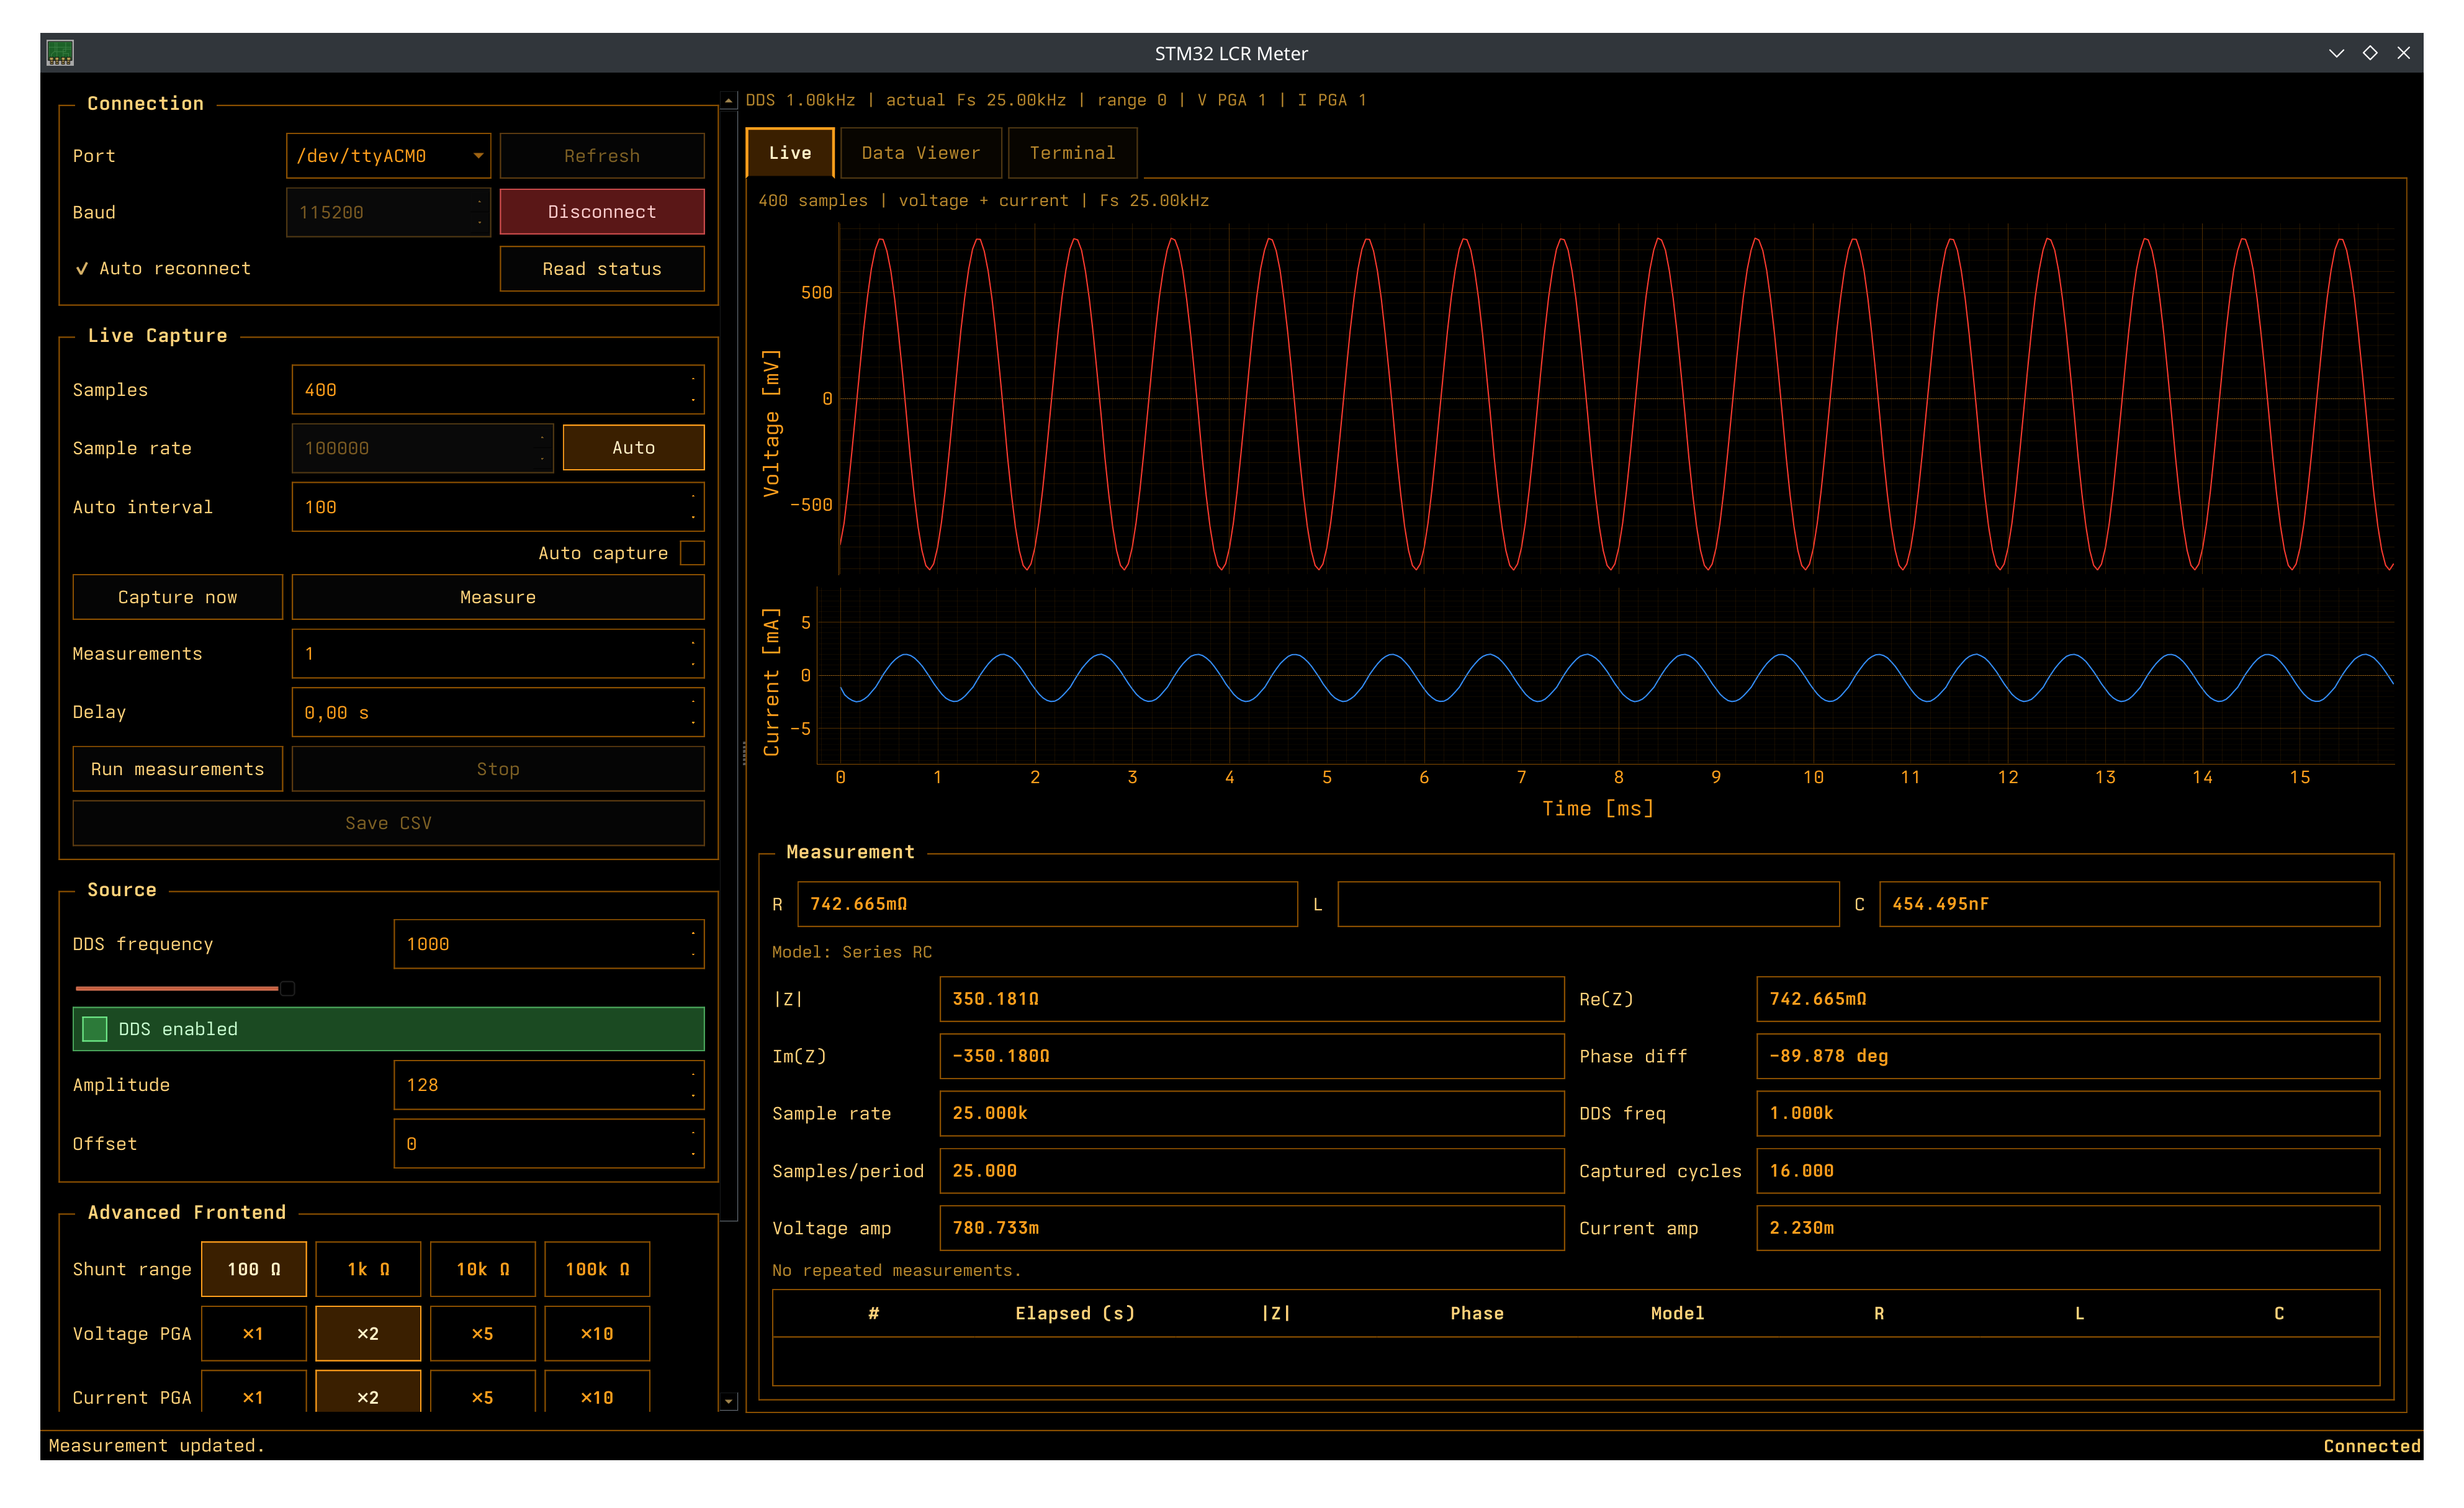
\includegraphics[width=\textwidth]{obrazky/basic_meas.png}
    \caption{Hlavní okno aplikace při základním měření}
    \label{fig:pc_app_basic_meas}
\end{figure}

V levé části aplikace jsou ovládací prvky přístroje, lze zde nastavit všechny parametry a odesílat příkazy měření.

Tlačítkem Capture now lze požádat o navzorkování napětí a proudu.
Tyto vzorky se náledně v pravé části zobrazí v osciloskopickém grafu.
Při aktivaci Auto capture je požadavek o vzorky odesílán periodicky, grafy se v čase aktualizují.

Jelikož v přístroji není implementována žádná funkce automatického nastavení rozsahu, je toto zobrazení
užitečné pro ruční nastavení. Čím větší je amplituda zobrazených grafů, tím přesněji přístroj měří.
Zároveň je vhodné na grafech zkontrolovat, zda není přítomné výrazné rušení nebo zda nejsou signály ořezané rozsahem ADC.

Tlačítko Measure také vede k navzorkování napětí a proudu, 
v tomto případě se do PC neposílají samotné vzorky ale již vypočítaná impedance.

Výsledky se zobrazí v pravé dolní části. Aplikace z impedance také odvodí hodnoty RC nebo RL. Výpočet probíhá podle vzorců:

\begin{equation}
    Z = R + jX
\end{equation}

\begin{equation}
    L = \frac{X}{2\pi f}, \quad \text{pro } X > 0
\end{equation}

\begin{equation}
    C = -\frac{1}{2\pi f X}, \quad \text{pro } X < 0
\end{equation}


\section{Statistické zobrazení}

Dále tato aplikace umožňuje automatizované mnohonásobné měření a následné statistické zpracování.
Tato funkce se spouští tlačítkem Run measurements po zadání množství měření a případného časového rozestupu mezi nimi.

Po dokončení měření se pravá část přepne na záložku Data Viewer, 
kde se zobrazí histogram a jemu přizpůsobená gaussova křivka.
Numerické statistické hodnoty jsou pak zobrazeny vlevo od grafu.

Naměřená data lze také uložit do souboru CSV, který pak lze v záložce Data Viewer opět otevřít.

\begin{figure}[H]
    \centering
    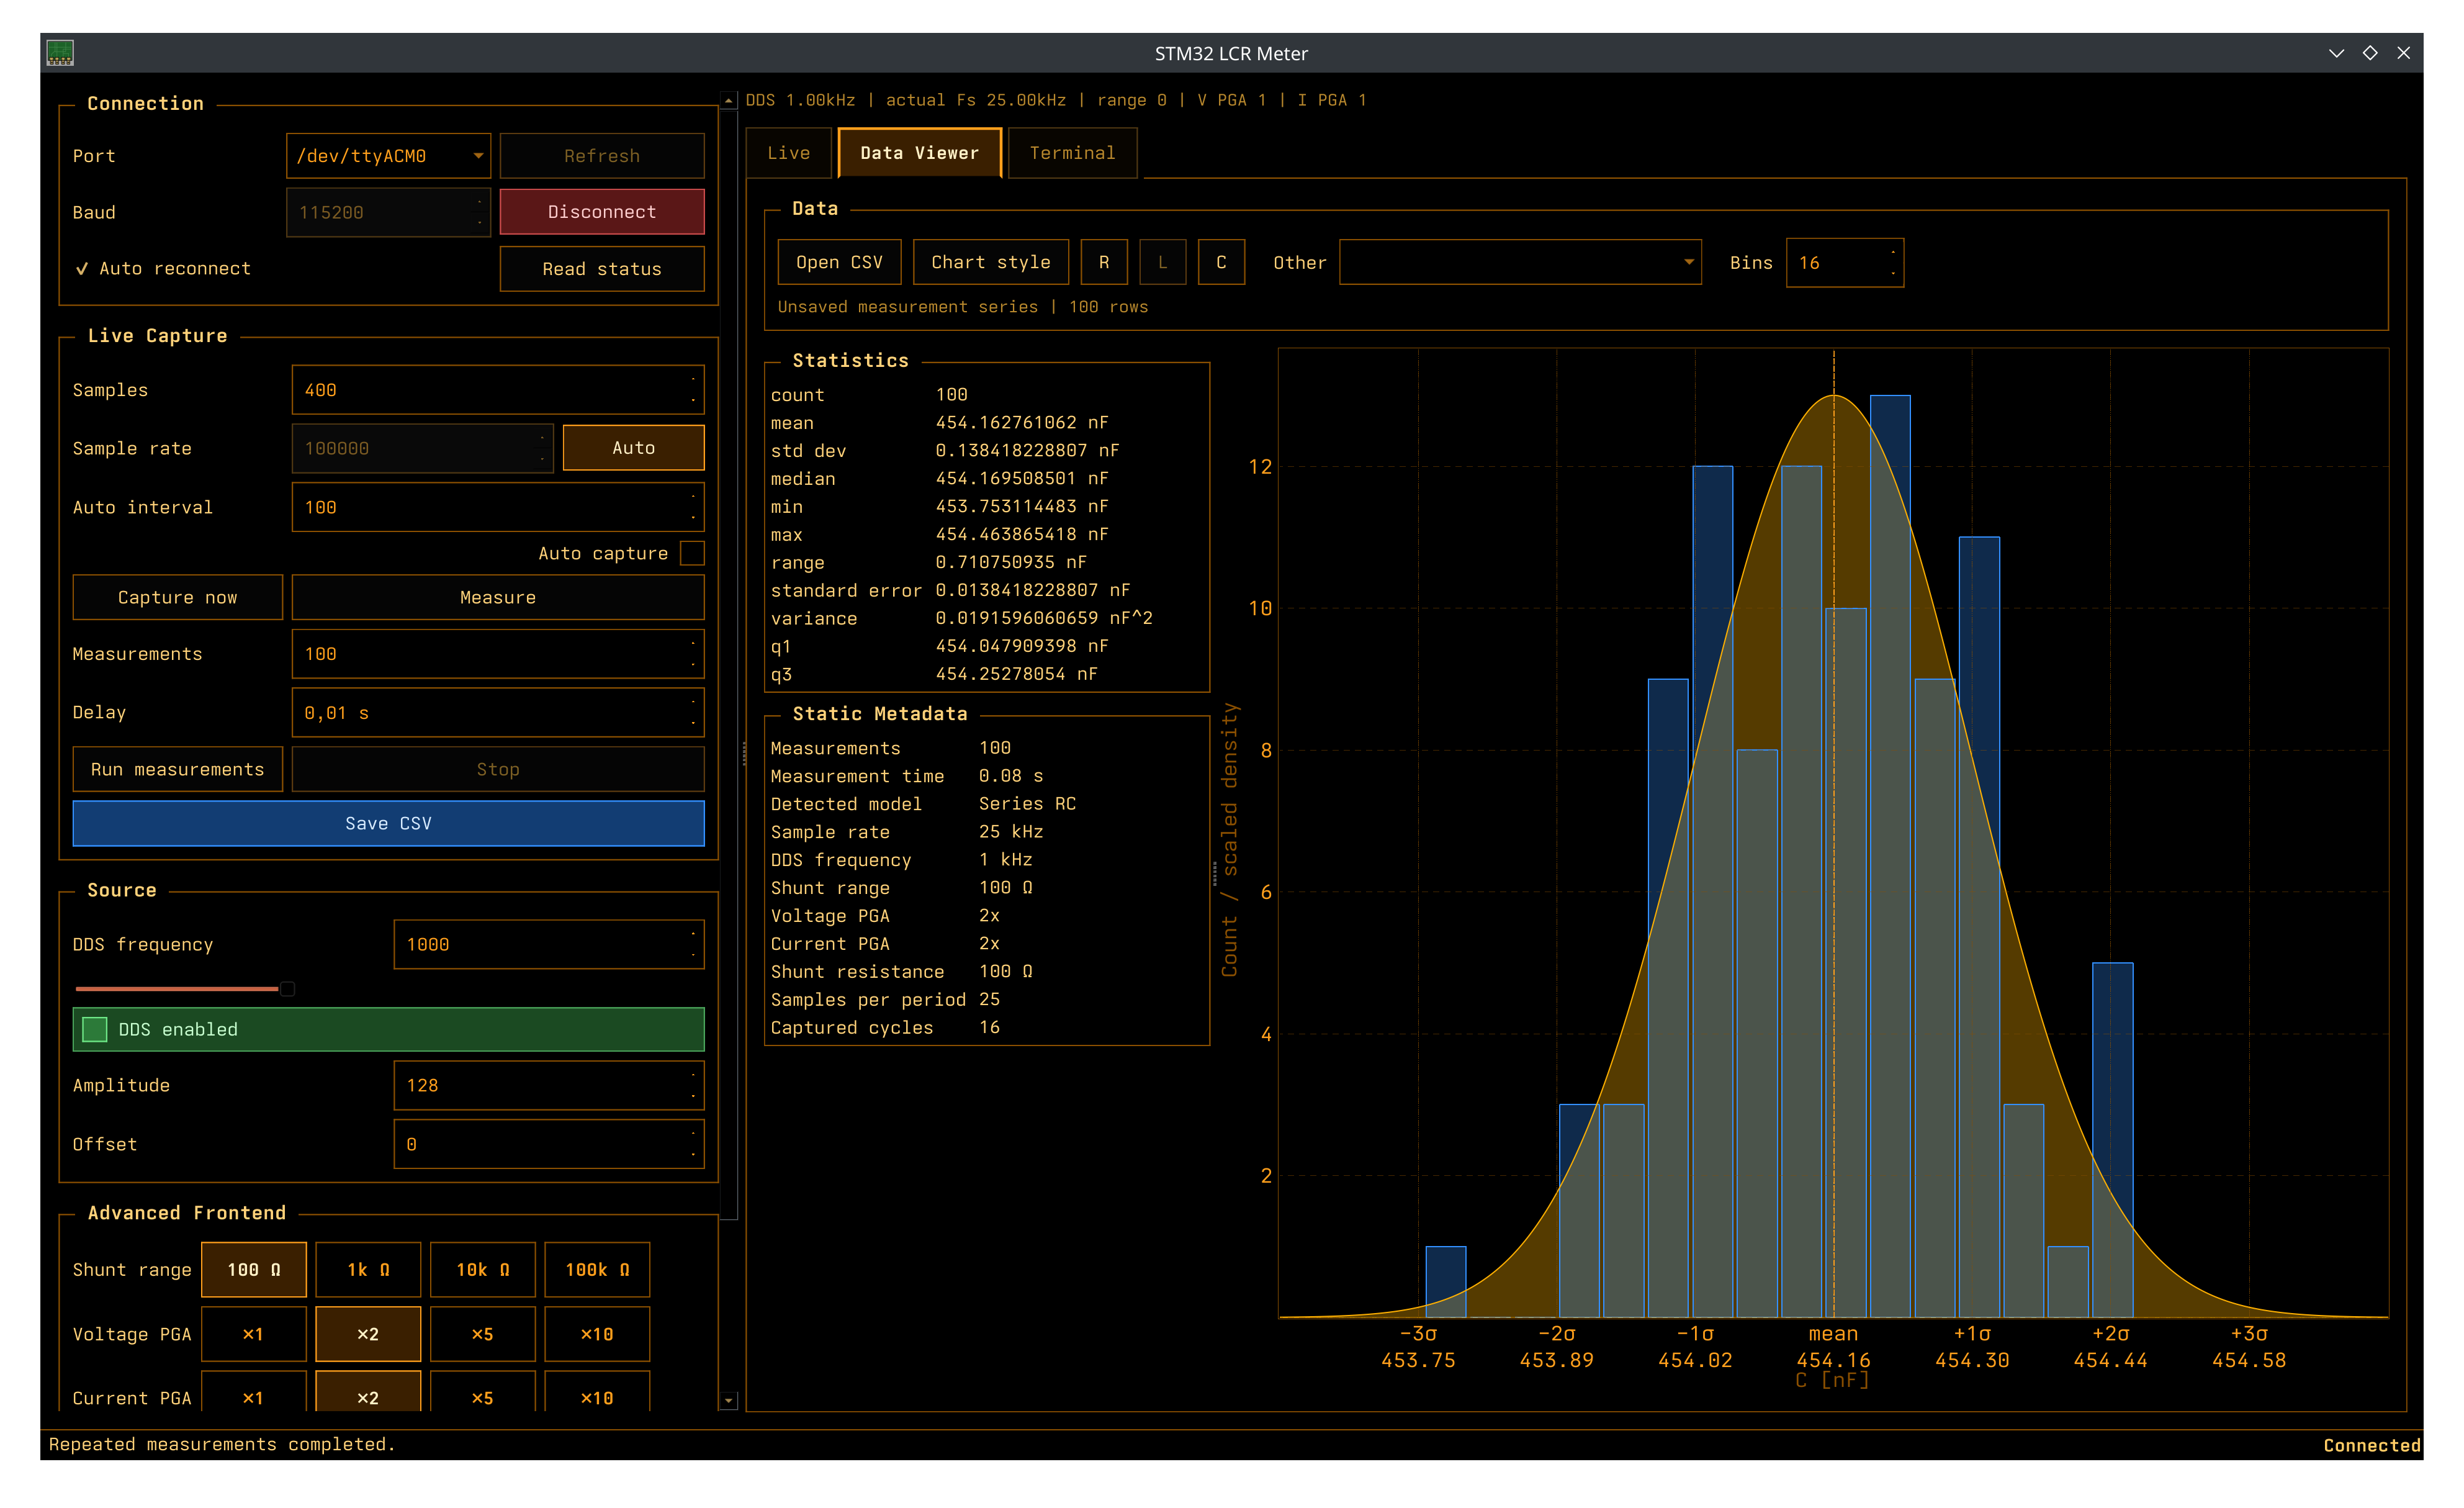
\includegraphics[width=\textwidth]{obrazky/stats_meas.png}
    \caption{Statistické zobrazení opakovaných měření v aplikaci}
    \label{fig:pc_app_stats_meas}
\end{figure}


\section{Integrovaný terminál}
Doplňkovou funkcí aplikace je záložka Terminal, 
která umožňuje nahlédnout na komunikaci se zařízením po sériové lince
a případňe ručně zadat příkaz. Při běžném použití to však není potřebné.

\begin{figure}[H]
    \centering
    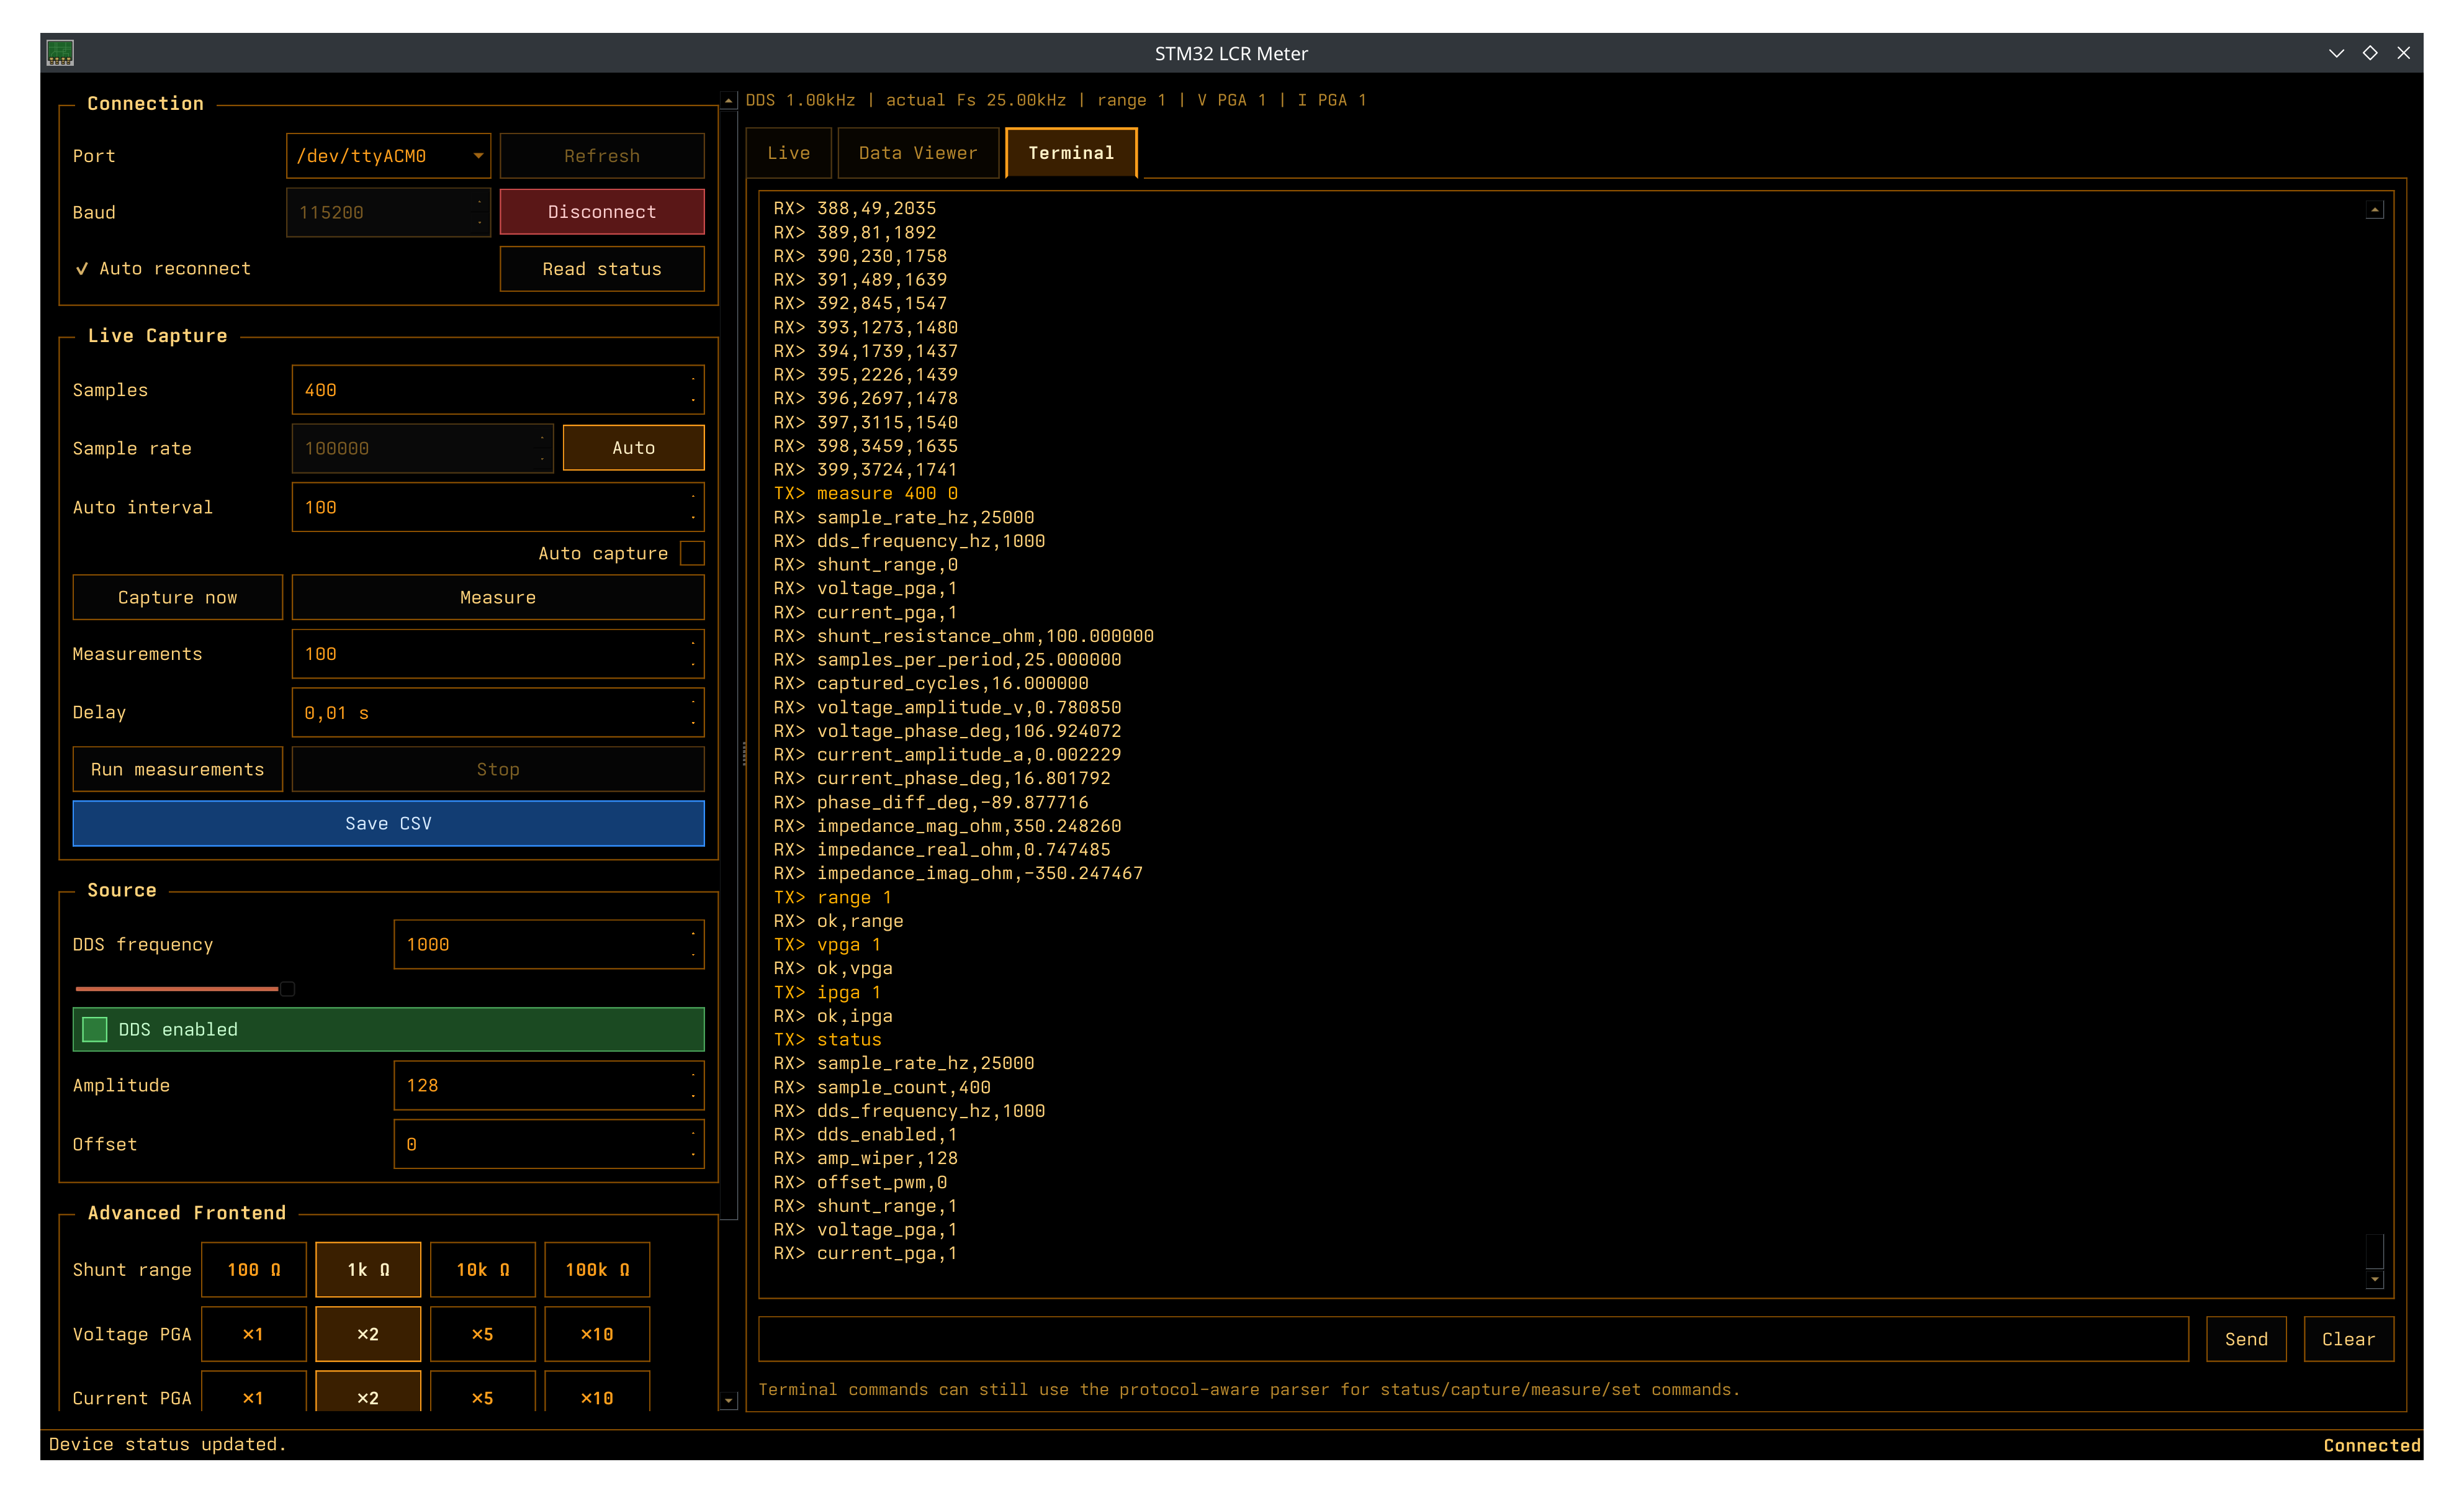
\includegraphics[width=\textwidth]{obrazky/integrovany_terminal.png}
    \caption{Integrovaný terminál aplikace pro ruční zadávání příkazů}
    \label{fig:pc_app_terminal}
\end{figure}
